%qqqqqqqqqqqqqqqqqqqqqqqqqqqqqqqqqqqqqqqqqqqqqqqqqqqqqqqqqqqqqqqqqqqqqqqqq
%Quote
\begin{savequote}[50mm]
%‘‘El cosmos es todo lo que es, todo lo que fue y todo lo que será. Nuestras 
%más ligeras contemplaciones del cosmos nos hacen estremecer: Sentimos como 
%un cosquilleo nos llena los nervios, una voz muda, una ligera sensación como
%de un recuerdo lejano o como si cayéramos desde gran altura. Sabemos que nos
%aproximamos al más grande de los misterios.’’
%\qauthor{Carl Sagan}
\end{savequote}
%qqqqqqqqqqqqqqqqqqqqqqqqqqqqqqqqqqqqqqqqqqqqqqqqqqqqqqqqqqqqqqqqqqqqqqqqq




%#########################################################################
%*****************************************************
\chapter{Modelo de Espín}
\label{cha:Modelo de Spin}
%*****************************************************

El espín\footnote{El espín hace alusión al momentum angular, para los BHs rotantes se hace uso de la métrica de Kerr.} de BH se sospecha que es un parámetro relevante para la dinámica de las galaxias, se cree que su importancia radica en parte a la dicotomía que existe entre radio loud AGNs y radio quiet AGNs. Este será el responsable de decir si existe alguna relación entre los AGNs y el entorno que habitan. En esta sección se presentarán los modelos que dan pie al origen, evolución y  alineamiento de los espines.

%===============================================
\section{Agujeros Negros Super Masivos (SMBHs)}
\label{sec: SMBH}
%================================================
Los SMBHs son objetos altamente masivos, que presenta un rango de masas entre $10^6M_{\odot}\lesssim M_{BH} \lesssim 10^{9}M_{\odot}$ \cite{mo2010}. Una de las evidencias que sugiere la existencia de los SMBHs, es que serían los causantes de la cantidad de energía que es emitida por los AGNs debido a la acreción de materia (mirar capitulo \ref{sec: Enigma_centarl}). Observaciones en regiones centrales de las galaxias, presentan un incremento en la razón masa-luminosidad, el cual no puede ser explicado por la presencia de poblaciones estelares, indicando que hay una objeto muy masivo, que no presenta una luminosidad considerable, permitiendo postular la existencia de un SMBH, ubicado en la parte central de la galaxia.  

La presencia de un SMBH en la galaxia solo influye dinámicamente en lugares cercanos a él (centrales). Usando la dispersión de las velocidades para estrellas cercanas al centro es posible encontrar un valor para la masa del objeto central, 

\begin{align}
    r_{BH}=\frac{GM_{BH}}{\sigma^{2}}
\end{align}
donde $\sigma$ es la dispersión de la velocidad, obtenida de medidas observacionales. 

En el contexto cosmológico se considera que todas las galaxias hospedan un SMBH en su interior, muy cercano al centro. Su existencia también viene arraigada por la misma teoría, son consecuencia de la relatividad general y de la teoría de formación de galaxias. 

La importancia de los SMBHs radica es su propiedad de acretar materia y convertirla en energía, esta energía liberada se conoce como feedback de agujero negro. Para galaxias grandes, el feedback es el responsable de que la galaxia deje de producir estrellas, debido a que este calienta el gas  impidiendo el colapso gravitacional por parte de las nubes de gas, y por ende impidiendo la formación estelar.

Yendo en dirección de poder conocer la información sobre el espín del BH o SMBH, es necesario saber cómo se originan y evolucionan. Es imperioso por tanto entender la teoría que abarca la evolución y crecimiento de los BHs.
%------------------------------------------------
\subsection{Crecimiento de SMBHs}
\label{subsec: Crecimiento_SMBHs}
%------------------------------------------------

El proceso de crecimiento de un SMBH esta determinado por la rata de acreción de masa. En la actualidad hay tres maneras posibles para el crecimiento del SMBH: fusión de BHs, colapso de nubes frías de gas que está alrededor galaxia y fusión entre galaxias \cite{fanidakis2011}. Cualquiera de estos tres sucesos pueden dar pie a la activación de un AGN, ya que este proceso es producto de la acreción súbita de materia. 
%-------------------------------------------------------
    \subsubsection{Fusión de BHs}
    \label{subsubsec: mergers_BHs}
%-------------------------------------------------------
La adquisición de materia por fusión entre BHs, corresponde a sistemas  binarios. La fricción dinámica que sienten los BHs  hace que estos pierdan momentum angular, dando como resultando una disminución en la separación entre ellos, y posteriormente repercutir en una fusión. También la perdida de energía debido a emisión de las ondas gravitacionales hace que la distancia entre los dos cuerpos se vaya reduciendo. A medida que pasa el tiempo 
la amplitud y por ende la energía de las ondas gravitacionales aumenta a medida que la separación entre los BHs binarios es menor.
%la emisión de las ondas gravitacionales es más consecutiva, haciendo que la perdida de energía sea mayor,
dando como resultado la coalescencia entre los dos BHs \cite{fanidakis2011}. 

%-------------------------------------------------------
    \subsubsection{Colapso de nubes de gas}
    \label{subsubsec: colapso_nubes_gas}
%-------------------------------------------------------
En galaxias de tipo temprano, donde es posible encontrar gas frío que esté en inmediaciones del centro de la galaxia, de tal forma que el gas pueda fluir directamente al BHs. Otra manera de acretar gas frío es por medio del método de radio-mode. Este mecanismo consiste en que el gas que es expulsado y calentado por la explosiones de supernovas o por el mismo SMBH, después de un largo tiempo se enfría y colapsa al centro de la galaxia, donde se encuentra el BH \cite{fanidakis2011}.

%-------------------------------------------------------
    \subsubsection{Colisión de galaxias}
    \label{subsubsec: mergers_galaxys}
%-------------------------------------------------------
La dinámica del universo y las observaciones, dejan ver que la interacción entre galaxias no es en nada extraño, siendo la colisión entre ellas un resultado esperado. Las galaxias espirales en su interior, en especial en la parte más interior del disco presentan una abundancia de gas frio, potencial para: la formación de estrellas, crecimiento de un BH y activación de un AGN. El proceso de fusión entre galaxias se distingue por fusiones mayores y menores\footnote{El proceso de fusión introduce un cambio en la morfología de las galaxias. Si es una fusión menor es posible que no altere la morfología de la galaxia más masiva, de manera considerable, mientras que las fusiones mayores transforma drásticamente la forma de las galaxias. }: las fusiones mayores indican colisiones donde la masa de los dos cuerpos son equivantes (Andromeda y Vía láctea), mientras en las fusiones menores la diferencia entre masas es considerable (Vía láctea y nube de magallanes). Cuando colisionan las dos galaxias, ya sea una fusión mayor o menor, producen un incremento en la formación estelar debido a la acumulación de gas frío de ambas galaxias. Pero no todo el gas frío se transforma en estrellas, parte de este cae al centro alimentando al BH.

%===============================================
\section{Evolución de espín}
\label{sec: Evolution_spin}
%===============================================

La evolución del espín del SMBH está altamente relacionada con la tasa de acreción de materia por parte del SMBH \cite{king2005}, y por la coalescencia de los BHs \cite{dubois2014}. Al considerar el interior de un AGN, se tiene entonces una estructura compuesta por un disco de acreción que orbita alrededor de un SMBH. Al suponer que tanto el SMBH como el disco de acreción rotan, implica un momentum angular (espín) tanto para el SMBH $\bf{J}_{bh}$, como para el disco de acreción $\bf{J}_{d}$. 
Los efectos relativistas producidos por el BH rotante, genera alrededor de él una torsión en el espacio-tiempo (Efecto Lense-Thirring).    
%Los torques de marea 
La torsión que actúan sobre ambos cuerpos rotantes conduce a alinear los espines, sin cambiar sus magnitudes \cite{king2005}.

El espín del SMBH puede ser definido como ${\bf{J}}_{bh}=|a|GM^{2}_{bh}/c$, donde $a$\footnote{normalizazión del momentum angular del BH.} es el parámetro de espín, acotado entre $-1\leq a \leq 1$: Sí $a=-1$ el BH está rotando en dirección contraría al disco de acreción, sí $a=1$ el BH y disco rotan en la misma dirección. ${\bf{J}}_{bh}$ juega un papel crucial para regiones cercanas al BH, indica la eficiencia de convertir la materia del disco en radiación, se cree además que su dirección está relacionada con la dirección del jet de AGN \cite{fanidakis2011}. 

%------------------------------------------------
\subsection{Acreción de gas}
\label{subsec: Acrecion_gas}
%------------------------------------------------
Como se expuso anteriormente, alrededor del SMBH existe un disco de acreción, que es originado por la conservación del momentum angular de una porción de gas  que caen al disco de acreción. Siguiendo lo propuesto por \cite{lynden1969}, las partículas que se encuentran el disco de acreción pierden momentum angular debido a torques producidos por los campos magnéticos, a medida que pierden momentum angular se van adentrando más en el disco, hasta llegar al borde interior del mismo. La orbita más interior es denominada como la ultima orbita estable (del ingles LSO). Sí la partícula se adentra en esta órbita será devorada con seguridad por el BH. El radio para la LSO en términos del momentum angular del BH se puede reescribir de la forma \cite{bardeen1972}:
%
\begin{align}
 \hat{r}_{lso}=\frac{r_{lso}}{R_g}=3+Z_{2}\pm \left[ (3-Z_{1})(3+Z_{1}+2Z_{2})\right]^{1/2} \,,
 \label{eq: radio_lso}
\end{align}
%
donde $R_{g}$ es el radio gravitacional, definido como la mitad del radio de Schwarzchild del BH, 
%
\begin{align}
    R_{g}= R_{schw}/2  = \frac{GM_{bh}}{c}\,.
\end{align}
%
Para valores de $a<0$ se toma el signo positivo de la ecuación (\ref{eq: radio_lso}), indicando que el BH rota de manera contraría al gas que están en la LSO, si $a>0$ se toma el signo negativo de la ecuación (\ref{eq: radio_lso}), obteniendo lo contrario, el BH rota en la misma dirección del gas. Los parámetros $Z_1$ y $Z_2$ se escriben de la forma:
%
\begin{eqnarray}
    Z_1 = 1+(1-a^{2})^{1/3}\left[(1+a)^{1/3}+(1-a)^{1/3} \right]\,,\\
    Z_2 = (3a^{2}+Z_{1}^{2})^{1/2}\,.
\end{eqnarray}
%
Un parámetro de gran importancia es la eficiencia radiativa del disco de acreción del BH $\epsilon_{r}$. Este parámetro indica la fracción de energía liberada por la materia que rota alrededor del BH. Al suponer un BH que rota, la eficiencia radiativa dependerá del parámetro de espín $a$ \cite{novikov1973}:
%
\begin{align}
    \epsilon_{r} \equiv 1- \sqrt{1-\frac{2}{3}\frac{1}{\hat{r}_{lso}(a)}}\,,
    \label{eq: eficiencia radiativa}
\end{align}
%
en otras palabras: entre más acreta menos irradia ó entre más irradia menos acreta.

A medida que el material cae a la LSO y posteriormente al BH, conlleva  una emisión de energía por unidad de masa $\widetilde{e}_{lso}$ y un momentum por unidad de masa $\widetilde{l}_{lso}$. Al considerar la masa contenida en una región muy cerca a LSO $dM_{0}$, permitiendo calcular el cambio de la masa y del momentum angular del BH, de la forma \cite{fanidakis2011}:
%
\begin{align}
    dM_{bh}=\frac{\widetilde{e}_{lso}}{c^{2}}dM_{0}, \, \, dJ_{bh}=\widetilde{l}_{lso}dM_{0}\,.
    \label{eq: dM_y_dJ}
\end{align}
%
La ecuación (\ref{eq: dM_y_dJ}) se relaciona con la ecuación para el espín del BH total ${\bf{J}}_{bh}$ de la forma:
%
\begin{align}
    \frac{da}{d\ln{M_{bh}}}=\frac{1}{M_{bh}}\frac{c^{3}}{G}\frac{\widetilde{l}_{lso}}{\widetilde{e}_{lso}}-2a\,,
\end{align}
%
La integral a esta solución es obtenida por \cite{bardeen1970}, dando como resultado: 
\begin{align}
    a^{f}=\frac{1}{3}\hat{r}_{lso}^{2}\frac{M_{bh}}{M_{bh}^{f}}\left[1- \left\{3\hat{r}_{lso}\left(\frac{M_{bh}}{M^{f}_{bh}} \right)^{2}-2 \right\}^{1/2} \right]\,,
    \label{eq: espin_final a^f}
\end{align}
donde $a^{f}$ y $M_{BH}^{f}$, corresponden al espín y masa final del BH. La ecuación (\ref{eq: espin_final a^f}) determina la evolución del espín $a$ durante el tiempo de acreción para un estado inicial. 

\begin{center}
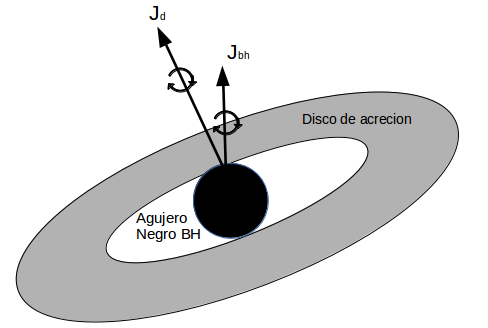
\includegraphics[scale=.35]{./figures/4_Modelo_Spin/Modelo_disco_bh.png}
\figcaption{\emph{Estructura del sistema BH y disco de acreción ambos rotantes y desalineados.}}\label{fig: desaliniamineto_bh_disco}
\end{center}

%------------------------------------------------
    \subsubsection{Acreción de gas en discos desalineados}
    \label{subsubsec: Acrecion gas desaliniado}
%------------------------------------------------
Siguiendo lo anteriormente expuesto, se tiene un disco de acreción que orbita alrededor de un BH. Los dos sistemas al estar rotando presentan un momemtum angular ${\bf{J}}_{bh}$ y ${\bf{J}}_{d}$. Gracias al análisis y resultados en \ref{subsec: Acrecion_gas} es posible asumir que la evolución del espín del BH, depende de la masa acretada por el mismo, ecuación (\ref{eq: espin_final a^f}). El proceso de acreción y cantidad de masa acumulada trasciende el análisis que se pretende realizar, sin embargo es posible tener un estimativo de estos procesos a partir de lo siguiente: Considerar el caso más general, donde se tiene que el disco de acreción rota en un plano diferente al plano ecuatorial del BH (los espines están desalineados), (ver figura \ref{fig: desaliniamineto_bh_disco}). Al considerar este sistema se tiene entonces, que el disco de acreción genera un torque debido al efecto Lense-Thirring (LT) producto de la rotación del BH. El efecto LT puede ser puede ser escrito de la forma:
%
\begin{align}
    \frac{\partial {\bf{L}}}{\partial t}={\bf{\Omega}}_{p}\times{\bf{L}}\,,
    \label{eq: lense-Thirring}
\end{align}
%
donde ${\bf{L}}$ es el momentum angular por unidad de área del disco y ${\bf{\Omega}}_{p}$ es rata de precesión, definida de la forma:
%
\begin{align}
    {\bf{\Omega}}_{p}=\frac{2G}{c^{2}}\frac{{\bf{J}}_{bh}}{R^{3}}\,,
\end{align}
%
donde $R$ es la distancia al BH \cite{pringle1992}. La viscosidad del disco determina altamente la evolución de los espines, entre más grande sea la viscosidad del disco, menor su tiempo de alineación, pero si es lo suficientemente alta, las partículas del interior generan otro disco deformado (warp) (ver figura \ref{fig: sistema con zona warp}), que se alinea con el espín del BH. Por tanto, se hace necesario introducir las escalas de tiempo que brindan información de la dinámica del sistema con alta viscosidad: Se introduce el tiempo de escala de acreción $t_{acc}\equiv R^{2}/\nu_{1}(R)$, indicando el tiempo que demora el gas del disco en caer al BH de manera paralela; el tiempo de escala warp $t_{warp}\equiv R^{2}/\nu_{2}(R)$, que equivale al tiempo de propagación de la deformación en dirección normal.  
%
\begin{center}
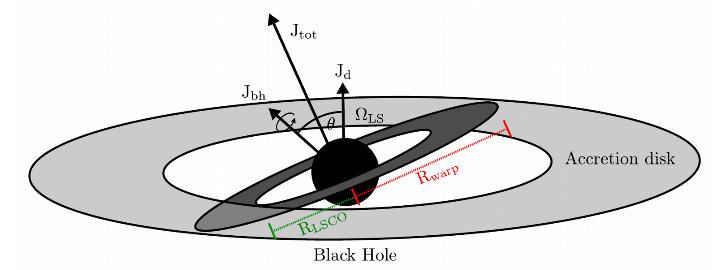
\includegraphics[scale=.4]{./figures/4_Modelo_Spin/Sistema_con_region_warp.png}
\figcaption{\emph{Esquema del sistema donde se ha dado una región warp. Se observan los diferentes espines de cada objeto, el radio warp, radio de la LSO. \cite{Bustamante2018b}}}\label{fig: sistema con zona warp}
\end{center}
%
Sin embargo, el plano ecuatorial del disco warp\footnote{disco interno que es deformado por los torque de marea producto de la alta viscosidad en el disco de acreción.} no mantiene la misma dirección, este precesa al rededor del plano ecuatorial de BH. El tiempo de precesión esta definido como:
%
\begin{align}
    t_{prec}= \frac{2\pi}{{\bf{\Omega}}_p(R)}\,.
\end{align}

Las escalas de tiempo permiten indicarnos si el torque producto del efecto LT, puede alinear los espines. La condición necesaria para el alineamiento es $t_{prec}\lesssim t_{warp}$ \cite{natarajan1999}. A partir de estas, es posible obtener el tamaño del disco deformado $R_{warp}$, en términos del radio de Schwarzschild $R_{Schw}$, el cual se puede escribir de la forma \cite{volonteri2007}:
%
\begin{align}
    \frac{R_{warp}}{R_{Schw}}=3.6\times 10^{3}a^{5/8}\left(\frac{M_{bh}}{10^{8}M_{\odot}} \right)^{1/8}f^{-1/4}\left(\frac{\nu_{2}}{\nu_{1}} \right)^{-5/8}\alpha^{-1/2}\,,
\end{align}
%
donde $f\equiv L/L_{Edd}$ es el radio de Eddington, $L_{Edd}=4\pi GM_{bh}c/\kappa$ es  la luminosidad de Eddington, con $\kappa\sim 0.3 [cm^{2}g^{-1}]$ siendo el scatering por opacidad de los electrones, y $L=\epsilon_{r}\dot{M}c^{2}$ es la luminosidad, con $\dot{M}$ la rata de acreción total y $\alpha$ es parámetro de viscosidad Shakura–Sunyaev.

La región warp\footnote{región deformada ubicada dentro del disco warp} proporciona bastante información sobre la evolución del BH. De esta región se puede inferir la cantidad de materia acretada por el BH $\dot{M_{bh}}$, la materia acretada lleva consigo momentum angular el cual también es consumido por el BH
%el cual sera transferido de manera directa como momentum angular
\cite{volonteri2007}. La masa warp se calcula a partir de $M_{warp}=\dot{M}t_{acc}(R_{warp})$, donde el tiempo de acreción en la región warp se calcula de la forma:
%
\begin{align}
 t_{acc}=\frac{R^{2}_{warp}}{\nu_{1}} = 3 \times10^{6}a^{7/8} \left(\frac{M_{bh}}{10^{8}M_{\odot}} \right)^{11/8}\times f^{-3/4}\left( \frac{\nu_{2}}{\nu_{1}}\right)^{-7/8}\alpha^{-3/2}\,\, \textit{yr}.
\end{align}
%
La relación entre las viscosidades $\nu_1$ y $\nu_2$ determina el tipo de proceso, acreción ó alineación del warp. Para un disco delgado se debe cumplir que $H/\alpha < a \ll 1$. En este trabajo se considera la relación $\nu_{2}/\nu_{1}=2(1+7\alpha)/(\alpha^{2}(4+a^{2}))$ \cite{ogilvie1999} , la cual cumple la condición $\nu_{2}/\nu_{1}\approx 1/\alpha^{2}$ \cite{papaloizou1983}. Bajo la relación asumida se obtiene que $t_{warp}< t_{acc}$, lo cual implica que el disco de la región warp se alinea con el plano ecuatorial del BH en una escala de tiempo menor que la escala de tiempo de acreción de masa. Anteriormente se había dicho que calcular la masa acretada por el BH no era trivial, sin embargo es posible suponer de muy buena manera que la masa warp equivale a la masa acretada en un único episodio $M_{d}$, al usar la ecuación (\ref{eq: Masa_acretada}) \cite{Bustamante2018b} se puede determinar la masa final del BH, necesaria para calcular la evolución del espín del BH (\ref{eq: espin_final a^f})
%
\begin{align}
 M_{d}= \frac{M_{bh}^{f}-M_{bh}}{1-\epsilon_{r}}\,.
 \label{eq: Masa_acretada}
\end{align}
%
%------------------------------------------------
    \subsubsection{Alineamiento o anti-alineamiento del espín}
    \label{subsubsec: Aling_Spin}
%------------------------------------------------

Los procesos que ocurren con respecto a la acreción de gas (sec \ref{subsec: Acrecion_gas}) determinan de una manera considerable la evolución del espín del sistema en general ${\bf{J}}_{tot}$. Recordando lo mencionado en la parte inicial de esta sección, se pude decir que el parámetro de espín $a$ también juega un papel importante en el proceso de alineamiento, proporcionando la dirección de rotación del sistema disco-BH. \cite{king2005} indica que para máxima contra-rotación\footnote{El BH rota en dirección contraria al disco} $a=-1$, con radio de orbita estable $r_{lso}=9$, y para máxima co-rotación\footnote{El BH rota en la misma dirección del disco} $a=1$ con $r_{lso}=1$ (ver figura \ref{fig: contra-rotacion y co-rotacion}). %se tiene entonces que a medida que aumenta $a$ disminuye $r_{lso}$ (ver figura \ref{fig: contra-rotacion y co-rotacion}). 
Al usar la ecuación (\ref{eq: eficiencia radiativa}) se obtiene que la eficiencia radiativa $\epsilon_{r}$ depende inversamente de $r_{lso}$ (ver figura \ref{fig: eficiencia_radiativa }), entonces si $r_{lso}$ crece, la eficiencia $\epsilon_{r}$ disminuye. Como ya se había expuesto, $\epsilon_{r}$ indica cuanta materia es expulsada en forma de energía, entonces conforme $\epsilon_{r}$ crece, menos aporta al momentum angular y al proceso de acreción del sistema. Por lo tanto al ser el sistema contra-rotante el que experimenta una eficiencia radiativa menor, producto del  gran tamaño de la orbita $r_{lso}$ (ver figura \ref{fig: eficiencia_radiativa }) 
%producto del signo de $a$
, es el proceso que más aporta al momentum angular y por ende a la evolución del espín. 

\begin{center}
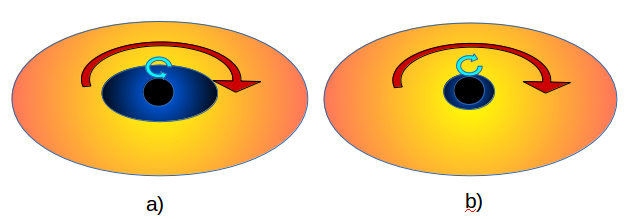
\includegraphics[scale=.35]{./figures/4_Modelo_Spin/Co-rotacion_contra-rotacion.png}
\figcaption{\emph{Comparación entre un sistema que co-rotante (b) y contra-rotante (a). Se observa que cuando es contra-rotante ($a\to -1$)} el radio $r_{lso}\to 9$, y de forma contraria si es co-rotante ($a\to 1$) el radio $r_{lso}\to 1$.}\label{fig: contra-rotacion y co-rotacion}
\end{center}
\begin{center}
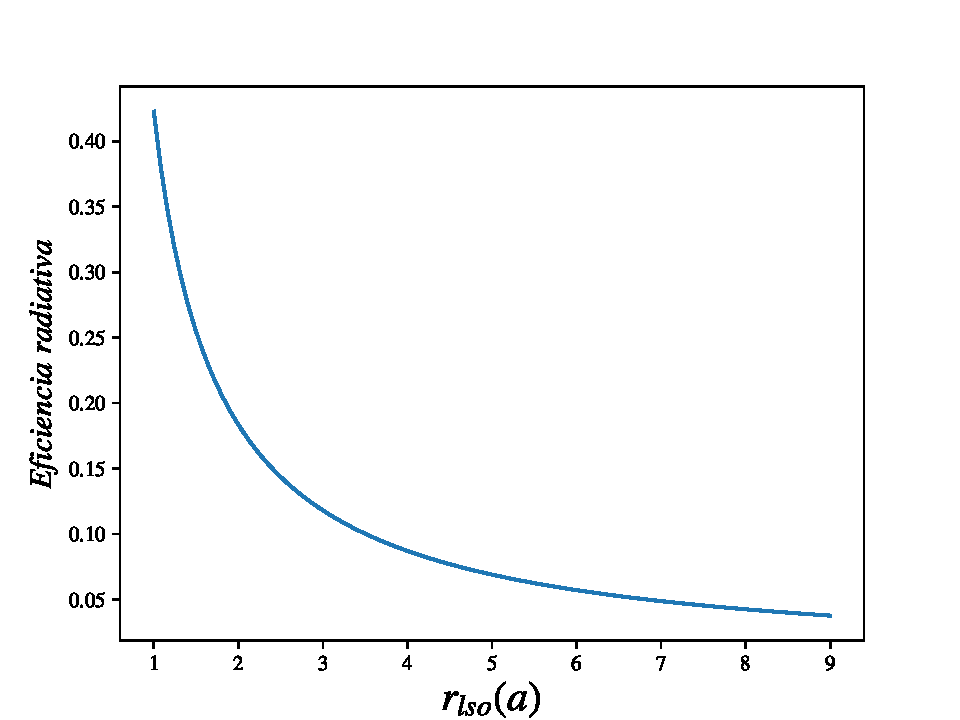
\includegraphics[scale=.5]{./figures/4_Modelo_Spin/eficiencia_radiativa.pdf}
\figcaption{\emph{Dependencia entre el radio de ultima orbita estable $r_{r}$ con la eficiencia radiativa $\epsilon_{lso}$, se observa que cuando $r_{lso}$ es mínimo la eficiencia es máxima, que corresponde a la máxima co-rotación $a=1$, indicando que gran parte del material se pierde y no contribuye al espín del sistema. Al observa el otro caso, pasa todo lo contario, siendo el sistema contra-rotante $a=-1$ el que mejor contribuye a la evolución del espín.}}\label{fig: eficiencia_radiativa }
\end{center}
%%************************
%SEria bueno poner las graficas de sebas sobre el la relación entre el tamaño de r, espin a y la eficiencia
%%*************************

Definiendo el espín del sistema de la forma:
\begin{align}
	{\bf{J}}_{tot}= {\bf{J}}_{bh}+{\bf{J}}_{d}
\end{align}
donde ${\bf{J}}_{d}$ es el momentum angular o espín del la región warp, se define el ángulo de desalineación $\theta$ como el resultado de  ${\bf{J}}_{bh}\cdot{\bf{J}}_{d}$, el cual está acotado ($-1\leq \cos\theta \leq 1$), donde si $\cos \theta \to -1$ indica un anti-alineamiento, y si $\cos \theta \to 1$ indica un alineamiento \cite{king2005}. Al considerar la derivada temporal del producto escalar de  ${\bf{J}}_{bh}$ se obtiene lo siguiente \cite{king2005}:
%
\begin{align}
    \frac{d }{dt}({\bf{J}}_{bh}\cdot {\bf{J}}_{bh})=  \frac{d}{dt}(J_{bh}^{2})= 0 \Rightarrow J_{bh}=cte\,.
\end{align}
%
Esta ecuación indica que ${\bf{J}}_{bh}$ se mueve sobre una esfera. Bajo la suposición anterior es posible concluir que el espín del BH se termina alineando con el espín total. 
%
\begin{align}
    \frac{d}{dt}(\cos\theta_{bh})\geq 0\,,
\end{align}
%
donde $\theta_{bh}$ es el ángulo entre ${\bf{J}}_{bh}$ y ${\bf{J}}_{tot}$, entonces $\theta_{bh}$ debe estar definido entre (0,$\pi/2$) para que se cumpla la condición de la derivada. Esta condición implica que siempre habrá un alineamiento, a medida que $\theta_{bh}$ disminuye en el tiempo, el $\cos\theta_{bh}$ aumenta, hasta llegar a su valor máximo ($\cos( 0)=1$) que indica un alineamiento definitivo.% lo cual implica que a medida que pasa el tiempo la diferencia entre los espines va disminuyendo, hasta llegar a alinearse.

Al saber eventualmente que el momentum angular total y el espín del BH se alinearan, proporciona gran información de la evolución del espín, sin embargo es necesario conocer si el espín del disco se terminara alineando o anti-alineando, para ello, miremos los criterios que dan cabida a ello. Partiendo de la magnitud del momentum angular total
%
\begin{align}
    J^{2}_{tot} = J^{2}_{bh}+J_{d}^{2} -2J_{bh}J_{d}\cos(\pi -\theta)
\end{align}
%
El anti-alineamiento ($\theta\to\pi$) ocurre si y solo si ${\bf{J}}_{bh}^{2}>{\bf{J}}_{tot}^{2}$, que equivale a \cite{king2005}:
%
\begin{align}
    \cos\theta < - \frac{{\bf{J}}_{d}}{2{\bf{J}}_{bh}}\,.   
\end{align}
%
Por lo tanto, gracias a este criterio es posible indicar si el sistema BH-disco está alineado/anti-alineado: si $\theta >\pi/2$ y $2{\bf{J}}_{bh}>{\bf{J}}_{d}$ el BH está anti-alineado, si  $2{\bf{J}}_{bh}<{\bf{J}}_{d}$ hay alineamiento, el cual siempre ocurre cuando el momentum angular del disco sobrepasa al del BH \cite{king2005}.

La magnidtud del momentum angular del disco esta dado por \cite{Bustamante2018b}:
%
\begin{align}
    J_{d}=\int_{warp} \Sigma_{d}\Omega_{k}(R)R^{2}dS \approx M_{d}(GM_{bh}R_{warp})^{1/2}\,,
    \label{eq: magnitid J_disco}
\end{align}
%
donde $\Sigma$ es la densidad superficial del disco, $\Omega_{k}$ es la frecuencia de Kepler y la integral va sobre todo la superficie de la región warp. Se ha asumido que todo el gas que va cayendo al BH esta circulando sobre todo el disco, entonces el momentum angular debería de distribuirse sobre toda la región warp. Este argumento permite encontrar una relación entre el momentum angular del disco y el BH \cite{king2005}.
%
\begin{align}
    \frac{J_{d}}{2J_{bh}}\approx \frac{M_{d}}{aM_{bh}}\left(\frac{R_{warp}}{R_{Schw}} \right)^{1/2}
\end{align}
%
Este criterio permite evaluar cada episodio de acreción, con lo cual se puede conocer si hay alineamiento o anti-alineamiento antes de que se acrete el disco [SEBAS]. 

\begin{center}
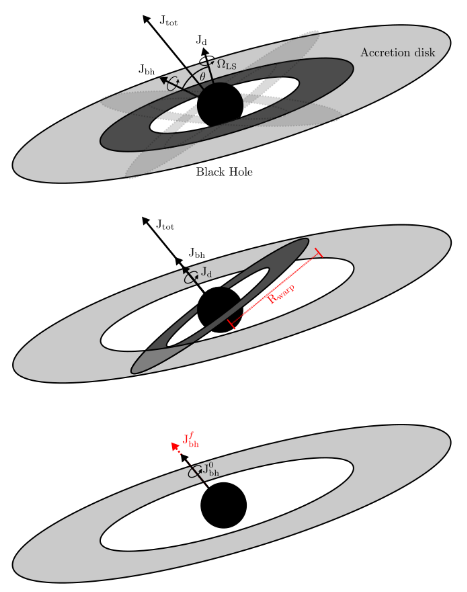
\includegraphics[scale=.5]{./figures/4_Modelo_Spin/evolucion_spin.png}
\figcaption{\emph{ Proceso evolutivo de los espines del sistema. En la figura superior, se tiene el caso inicial donde se formó la región warp, la cual está precesando. La figura del medio presenta el momento en que la región warp se estabiliza, alineando su espín con el espín del BH. La figura inferior muestra el momento final, donde todo los espines se alinean y la masa del disco interno ha sido acretada  \cite{Bustamante2018b}.}}\label{fig: evolucion espin}
\end{center}


%------------------------------------------------
    \subsubsection{Discos auto-gravitantes}
    \label{subsubsec: Disco auto-gravitantes}
%------------------------------------------------
Cuando se llega al caso en el cual la rata de acreción del sistema BH y disco de acreción es muy alta, se genera un disco de acreción aun más grande. En las regiones más externas del disco de acreción se empiezan a formar una zona donde la gravedad  es comparable o mayor al potencial gravitacional generado por el BH, permitiendo el colapso de pequeñas parcelas de gas
%grueso, que al no estar tan cerca al BH, sienten una gravedad propia y empieza a colapsar en pequeñas nubes de gas 
(figura \ref{fig: Sistema auto-gravitante}). Esta región externa comienza a formar estrellas muy masivas que evolucionan rápidamente, que al explotar como súper novas generan vientos  violentos que perturban el sistema, en especial que afectan la dinámica del disco interior de forma caótica. 
%
\begin{center}
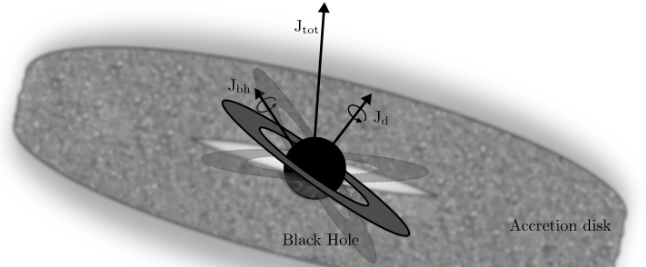
\includegraphics[scale=.3]{./figures/4_Modelo_Spin/Sistema_auto-gravitante.png}
\figcaption{\emph{Modelo del sistema auto-gravitante, en la parte exterior a la región warp se forma una distribución de gas, la cual es gobernada por una dinámica auto-gravitante \cite{Bustamante2018b}.}}\label{fig: Sistema auto-gravitante}
\end{center}
%
Para entender este suceso se hace uso del criterio de estabilidad de Toomre, el cual compara el soporte rotacional del disco contra su propia gravedad \cite{Bustamante2018b}:
%
\begin{align}
    Q\equiv\frac{c_{s}\Omega_{k}}{\pi G\Sigma_{d}}\,,
    \label{eq: estabilidad_Toomre's}
\end{align}
%
%
donde $c_{s}$ es la velocidad del sonido en el gas. En el caso en que $Q\leq 1$ el disco es inestable, esto conduce a la definición un radio de auto-gravedad $R_{sg}$, el cual debe cumplir que $Q(R_{sg})=1$. El radio de auto-gravedad es determinado por \cite{fanidakis2011}:
\begin{align}
    \frac{R_{sg}}{R_{Schw}}=1.5\times 10^{3}\epsilon^{8/27}\left(\frac{M_{bh}}{10^{8}M_{\odot}} \right)^{-26/27}f^{-8/27}\alpha^{14/27}
\end{align}
%
Debido a que $Q$ es un parámetro que decrece monótonamente a medida que crece el radio, la parte exterior al $R_{sg}$, donde no se cumple el criterio de estabilidad de Toomre, esta sujeta a fragmentación, mientras que la parte interior que sí se cumple la condición se genera un disco estable. Solo el material que se encuentra dentro del radio de warp puede transferir momentum angular de forma eficiente, es por eso que solo se incluye los efectos de auto-gravedad si $R_{sa}\leq R_{warp}$. Si se cumple la relación anterior, se debe obtener la relación de la masa que contribuye al momentum angular del sistema, dada por \cite{fanidakis2011}:
%
\begin{align}
    M_{sg} = 2.13\times 10^{5}\epsilon^{-5/27}\left(\frac{M_{bh}}{10^{8}M_{\odot}} \right)^{23/27}f^{5/27}\alpha^{-2/17}M_{\odot}\,.
\end{align}
%
Ahora con los valores de $M_{sg}$ y $R_{sg}$ que al remplazarlos por $M_{d}$ y $R_{warp}$, se puede obtener la evolución del espín del BH en el régimen de auto-gravedad.


%------------------------------------------------
\subsection{Coalesencia de BH's}
\label{subsec:fusion_BHs}
%------------------------------------------------
La otra forma de poder cambiar la dirección y magnitud del espín del BH es a partir de fusiones entre  sistemas binarios de BHs (ver figura \ref{fig: fusion_Bhs}). Este fenómeno es común en procesos de formación jerárquicos, en los cuales dos galaxias colisionan, generando un pozo de potencial donde los dos BHs perteneciente a cada galaxia van a terminar cayendo, y posteriormente fusionándose debido a la fricción dinámica. Entonces al fusionarse los dos BHs, la dirección de cada uno se combina, generando un nuevo espín. Una forma de calcular el espín resultante de la fusión, es usando el ajuste analítico de \cite{rezzolla2008}: 
%
\begin{align}
    a = \frac{1}{(1+q)^{2}}(a_{1}+a_{2}q^{2}+\ell q)\,,
\end{align}
%
donde $a_{1}$ es el parámetro de espín del BH más masivo, $a_{2}$ equivale al parámetro de espín del menos masivo, $q$ es la razón entre las masas $q=M_{2}/M_{1}\leq 1$ y $ {\bf{\ell}} = {\bf{l}}/(M_{1}M_{2})$, donde ${\bf{l}}$ es la diferencia entre el momentum angular orbital ${\bf{L}}$ con el momentum angular de las ondas gravitacionales ${\bf{J}}_{og}$, en un instante antes de la fusión ${\bf{l}}={\bf{J}}-{\bf{J}}_{og}$.

La norma de $\ell$ se obtiene de forma analítica \cite{rezzolla2008}: 
%
\begin{align}
    \ell = \frac{s_{4}}{(1+q^{2})^{2}}(a_{1}^{2}+a_{2}^{2}q^{4}+2{\bf{a_{1}\cdot a_{2}}}q^{2})\\ + \frac{s_{5}\mu + t_{0}+2}{1+q^{2}}(a_{1}\cos\phi_{1}+a_{2}q^{2}\cos\phi_{2})\\ 
    + 2\sqrt{3}+t_{2}\mu+t_{3}\mu^{2}\,,
\end{align}
donde $\phi_{1}(\phi_{2})$ son los ángulos entre $a_{1}(a_{2})$ y $\vec{\ell}$, y $\mu = q/(1+q)^{2}$. Al igual que supone \cite{rezzolla2008}, se considera que la dirección de $\Vec{\ell}$ es paralela con la dirección del momentun angular ${\bf{L=L_{1}+L_{2}}}$ antes de la fusión, el cual es un vector medido en la simulación. Para tener el valor de ${\bf{L}}$ es necesario calcular el centro de masa del sistema binario ${\bf{r}}_{com}$, con esta posición se evalúa el momentum angular de los dos BHs relativo al centro de masa. Se tiene además los valores de los coeficientes: $s_{4}=-0.129$, $s_{5}=-0.384$, $t_{0}=-2.686$, $t_{2}=-3.454$ y $t_{3}=2.353$ \cite{rezzolla2008}.

\begin{center}
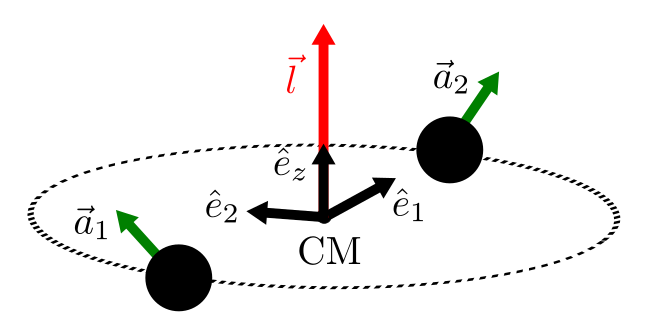
\includegraphics[scale=.3]{./figures/4_Modelo_Spin/fusion_BHs.png}
\figcaption{\emph{Sistema binario de BHs, donde cada uno tiene un espín característico y la contribución de cada uno conlleva a un momentum angular del sistema $\vec{\ell}$ \cite{Bustamante2018b}}.}\label{fig: fusion_Bhs}
\end{center}















%*************************************************************************